\documentclass[11pt]{article}
\usepackage[utf8]{inputenc}
\usepackage[T1]{fontenc}
\usepackage{grffile}
\usepackage{longtable}
\usepackage{wrapfig}
\usepackage{rotating}
\usepackage[normalem]{ulem}
\usepackage{amsmath}
\usepackage{textcomp}
\usepackage{amssymb}
\usepackage{capt-of}
\usepackage{hyperref}
\hypersetup{colorlinks=true, linkcolor=magenta}
\setlength{\parindent}{0in}
\usepackage[margin=0.8in]{geometry}
\usepackage[english]{babel}
\usepackage{mathtools}
\usepackage{palatino}
\usepackage{fancyhdr}
\usepackage{sectsty}
\usepackage{engord}
\usepackage{parskip}
\usepackage{minted}
\usepackage{cite}
\usepackage{graphicx}
\usepackage{subcaption}
\usepackage{setspace}
\usepackage[compact]{titlesec}
\usepackage[center]{caption}
\usepackage{placeins}
\usepackage{color}
\usepackage{amsmath}
\usepackage{bm}
\usepackage{todonotes}
\usepackage{pdfpages}
% \titlespacing*{\subsection}{0pt}{5.5ex}{3.3ex}
% \titlespacing*{\section}{0pt}{5.5ex}{1ex}
\author{Luis Antonio Ortega Andrés\\Antonio Coín Castro}
\date{}
\title{Face Biometrics Lab - Report}
\hypersetup{
 pdfauthor={Luis Antonio Ortega Andrés, Antonio Coín Castro},
 pdftitle={},
 pdfkeywords={},
 pdfsubject={},
 pdflang={Spanish}}}

\begin{document}

\maketitle

\section*{Exercise 1}

\textit{Based on the provided code, run the \texttt{FaceRecognition.m} file and complete the following points.}

\textbf{a)} \emph{Paste one image of the ATT Face Dataset and the corresponding image after using the 2D Discrete Cosine Transform (DCT)}.

The results are shown in Figure \ref{fig:ex1a}, where we use the default value of $10$ coefficients for the DCT. The image on the right is a representation of the image on the left using a few \textit{basis functions} (cosine waves).

\begin{figure}[h!]
  \centering
       \begin{subfigure}[t]{0.4\textwidth}
         \centering
         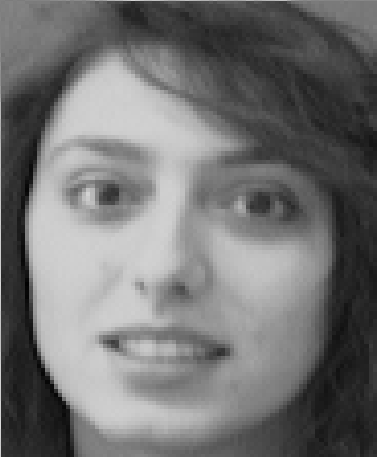
\includegraphics[scale=0.4]{img/1a_orig}
         \caption{Original image}
     \end{subfigure}%
     \quad
     \begin{subfigure}[t]{0.4\textwidth}
         \centering
         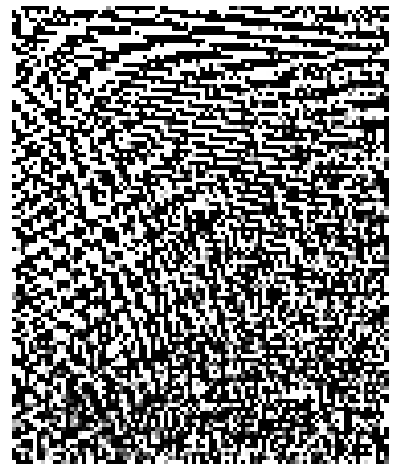
\includegraphics[scale=0.4]{img/1a_dct}
         \caption{DCT representation}
     \end{subfigure}
    \caption{Sample face image before and after applying DCT.}
    \label{fig:ex1a}
\end{figure}

\textbf{b)} \emph{Using the original configuration parameters (train = 6 images, test = 4 images, DCT coefficients = 10), plot the resulting DET image and indicate the resulting EER.}

The resulting DET curve is shown in Figure \ref{fig:ex1b}. The EER achieved, marked with a circle on the image, is $5.6891\%$. Recall that this value represents the point where the false acceptance rate and false rejection rate are equal.

\begin{figure}[h!]
  \centering
    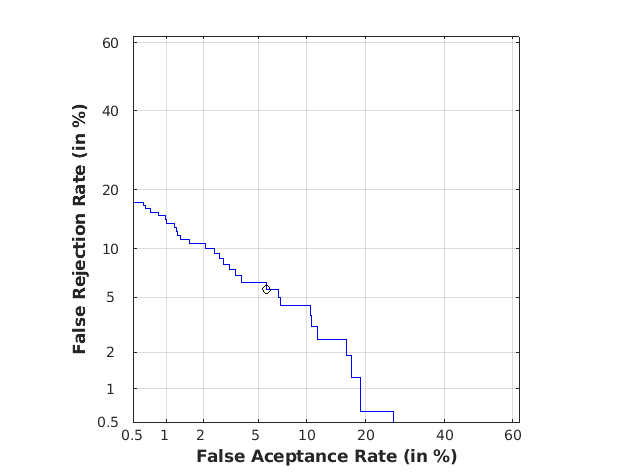
\includegraphics[scale=0.6]{img/1b_det}
    \caption{DET curve obtained with default parameters.}
    \label{fig:ex1b}
\end{figure}

\textbf{c)} \emph{Find out the configuration of the DCT coefficients that achieves the best EER results (keeping train = 6 images, test = 4 images). Justify your result, including the resulting DET image and EER value.}

Since we know that in general most images can be represented with just a few of the first DCT coefficients, we explore the best configuration in the search space in which the number of coefficientes varies from $1$ to $20$. The best EER result was $3.75\%$, obtained with \textit{coeff=5}, and the corresponding DET curve can be seen in Figure \ref{fig:ex1c}. We have achieved an EER that is about 2 percentage points smaller than the one obtained with the default parameters.

\begin{figure}[h!]
  \centering
    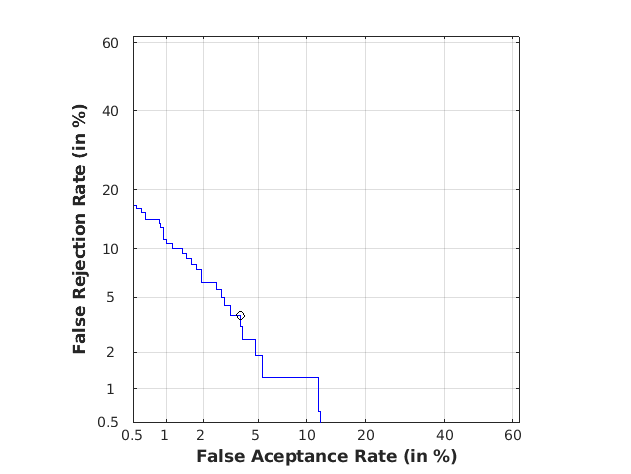
\includegraphics[scale=0.6]{img/1c_det}
    \caption{DET curve obtained with \textit{coeff=5}.}
    \label{fig:ex1c}
\end{figure}

Next we show in Figure \ref{fig:ex1c_bis} a comparison of the DET curves for all values \textit{coeff}$=1,\dots,20$, and also the evolution of the EER values with respect to the \textit{coeff} parameter.

\begin{figure}[h!]
  \centering
       \begin{subfigure}[t]{0.4\textwidth}
         \centering
         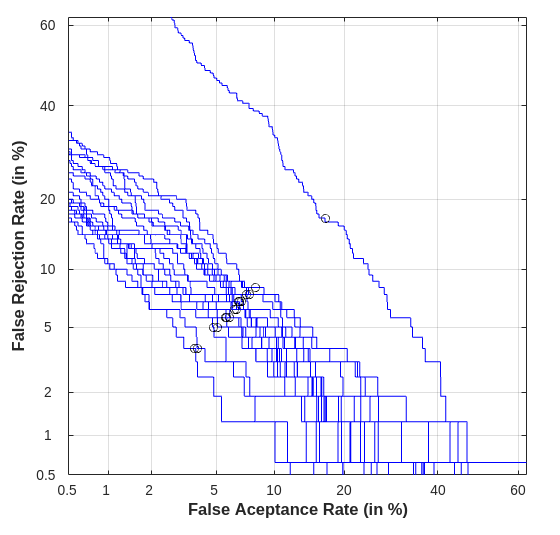
\includegraphics[scale=0.4]{img/1c_det_all}
         \caption{DET curves}
     \end{subfigure}%
     \quad \quad
     \begin{subfigure}[t]{0.4\textwidth}
         \centering
         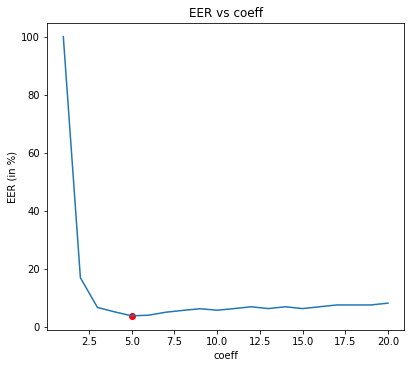
\includegraphics[scale=0.6]{img/1c_eer_evol}
         \caption{EER evolution}
     \end{subfigure}
    \caption{DET and EER for all values of \textit{coeff}.}
    \label{fig:ex1c_bis}
\end{figure}

\newpage
\textbf{d)} \textit{Once the best configuration of the DCT coefficients has been selected (in previous point), analyze the influence of the number of training images in the system performance. Include the EER result achieved for each case (from train = 1 to train = 7). Justify the results.}

We fix the parameter \textit{coeff}$=5$. Varying the value of \textit{train} from $1$ to $7$ (and setting \textit{test} to $10-$\textit{train}), the best EER result achieved was $3.3333\%$, obtained with \textit{train=7}, and the corresponding DET curve can be seen in Figure \ref{fig:ex1d}. As we can see, we have succeeded in lowering the EER obtained in \textbf{1c)}.

\begin{figure}[h!]
  \centering
    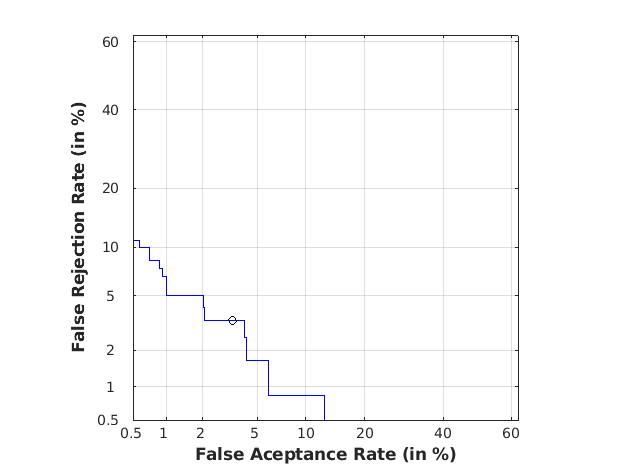
\includegraphics[scale=0.6]{img/1d_det}
    \caption{DET curve obtained with \textit{train=7}.}
    \label{fig:ex1d}
\end{figure}

The EER values obtained for each value of \textit{train} are summarized in Table \ref{tab:ex1d}, and a graph showing the evolution is shown in Figure \ref{fig:ex1d_bis}. The conclusion we draw is that a $70\%-30\%$ split in the dataset leads to better results regarding the EER.

\begin{table}
  \centering
  \begin{tabular}{c|ccccccc}
    \textbf{Train} & 1 & 2 & 3 & 4 & 5 & 6 & 7\\
    \hline
    \textbf{EER (\%)} & 13.0556 & 9.3750 & 6.4286 & 5.8333 & 5.0000 & 3.7500 & 3.3333
  \end{tabular}
  \caption{EER values obtained for each value of \textit{train}.}
  \label{tab:ex1d}
\end{table}

\begin{figure}[h!]
  \centering
    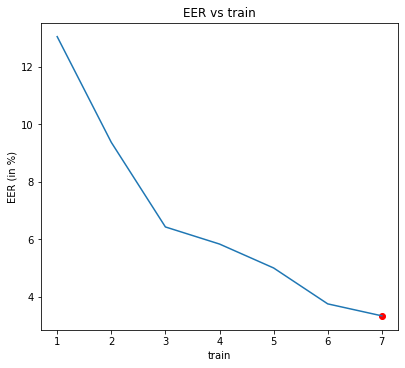
\includegraphics[scale=0.6]{img/1d_eer_evol}
    \caption{EER evolution for different values of the \textit{train} parameter.}
    \label{fig:ex1d_bis}
\end{figure}

\section*{Exercise 2}

\textit{The goal of this task is to change the feature extraction module. Instead of using DCT coefficients as in Task 1, you must consider \textbf{Principal Component Analysis (PCA)} to extract more robust features.}

%You can use the pca.m function available in Matlab. For the training phase, you should follow:
%[coeff_PCA,MatrixTrainPCAFeats,latent] = pca(MatrixTrainFeats);
%meanTrainMatrix=mean(MatrixTrainFeats);
%It is important to remark that the PCA function must be applied once for all training users and samples (not one PCA per user as this would provide specific coeff_PCA parameters per user).
%For the test phase, you should follow:
%For each test, subtract the meanTrainMatrix, and multiply by the coeff_PCA transformation matrix in order to obtain the test features in the PCA domain.
%For more information, check Matlab Help: https://es.mathworks.com/help/stats/pca.html

\textbf{a)} \emph{Using the parameters train = 6 and test = 4, paste the DET curve and indicate the EER when using all the PCA components.}

\textbf{b)} \emph{A key aspect for PCA is the number of components considered. Analyze and represent how the EER value changes in terms of the number of PCA components. Give your explanation about the results achieved.}

\textbf{c)} \textit{Indicate the optimal number of PCA components and paste the resulting DET curve together with the EER achieved. Compare the results using PCA with the DCT features considered in Task 1.}

\section*{Exercise 3}

\textit{The goal of this task is to improve the matching module. Instead of using a simple distance comparison, you must consider Support Vector Machines (SVM). In this case, you should train one specific SVM model per user using the training data (train = 6 images). Features extracted using the PCA module developed in Task 2 must be considered in this Task.}

%You can use the fitcsvm function available in Matlab. For the training phase, you should follow:
%SVMModel = fitcsvm(…)
%For the test phase, you should follow:
%[label,score]= predict(SVMModel,MatrixTestFeats);
%to obtain the scores for each user model.
%For more information, check Matlab Help:
%https://es.mathworks.com/help/stats/fitcsvm.html?lang=en

\textbf{a)} \emph{Using the parameters train = 6 and test = 4, paste the DET curves and indicate the EERs in the following cases: 1) regarding the KernelFunction parameter of the SVM (using all PCA components), and 2) regarding the number of PCA components considered for the feature extraction module (using the KernelFunction polynomial and starting with 3 PCA components).}

\end{document}
